\chapter{Flujo en Redes}
\label{flujo}

\section{Flujo máximo}

Una \textit{red de flujo} es un digrafo $N = (V, E)$ junto con una función de \textit{capacidad} $u: E \longrightarrow \Z_+$ y un par de nodos $s, t \in V$, llamados origen y destino. Un \textit{flujo factible} $x: E \longrightarrow \Z_+$ en esa red es una asignación de valores a las aristas, de forma que se cumpla:
\begin{itemize}
    \item $0 \leq x(v_i \rightarrow v_j) \leq u(v_i \rightarrow v_j)$ (Respeta las capacidades).
    \item $\forall v_i \in V - \{s, t\},$
          \begin{flalign*}
               &  & \sum_{u \in N^+(v)} x(u \rightarrow v) = \sum_{u \in N^-(v)} x(v \rightarrow u) &  & \textit{(Conservación)}
          \end{flalign*}
\end{itemize}


El \textit{valor del flujo} $x$ es la cantidad neta que sale del vértice $s$, es decir:
$$F = \sum_{u \in N^+(s)} x(u \rightarrow s) - \sum_{u \in N^-(s)} x(s \rightarrow u)$$

Entonces, se puede definir el problema de flujo máximo:

\begin{problema}
    Dada una red de flujo $N = (V, E, u)$ con origen $s$ y destino $t$, encontrar un flujo factible $x$ que tenga valor $F$ máximo. Es decir, maximizar:
    $$F = \sum_{u \in N^+(v)} x(u \rightarrow s) - \sum_{u \in N^-(v)} x(s \rightarrow u)$$

    Sujeto a:
    \begin{itemize}
        \item $0 \leq x(e) \leq u(e)\ \forall e \in E$
        \item $\forall v_i \in V - \{s, t\},$
              $$\sum_{u \in N^+(v)} x(u \rightarrow v) = \sum_{u \in N^-(v)} x(v \rightarrow u)$$
    \end{itemize}
\end{problema}

Las unidades del flujo se pueden considerar ``paquetes'' que viajan del origen $s$ al destino $t$, donde cada paquete puede tomar cualquier ruta que tenga la capacidad necesaria.

\subsection{Corte}

Un \textit{corte} en una red de flujo $N = (V, E, u)$ es un subconjunto $S \subseteq V$ tal que $s \in S$ y $t \notin S$. Por otro lado, dado un par de subconjuntos $S, T \subseteq V$, se define:
$$ST = \{u \rightarrow v \mid u \rightarrow v \in E, u \in S, v \in T\}$$

\begin{theorem*}
    \leavevmode

    Sea $x$ un flujo definido en una red $N = (V, E, u)$ y sea $S$ un corte. Entonces:
    $$F = \sum_{e \in S\bar{S}} x(e) - \sum_{e \in \bar{S}S} x(e)$$

    Donde $\bar{S} = V - S$.
\end{theorem*}
\begin{proof}
    Sumando los flujos netos que pasan por los vértices de $S$, se obtiene:
    $$\sum_{v \in S}\underbrace{\left(\sum_{u \in N^+(v)} x(u \rightarrow v) - \sum_{u \in N^-(v)} x(v \rightarrow u)\right)}_{\text{Siempre $0$, excepto para $v = s$}} = F + 0$$

    Por otro lado, los términos de la sumatoria representan todas las aristas que conectan un nodo de $S$ con uno de $V$, así que:
    $$F = \sum_{e \in SV} x(e) - \sum_{e \in VS} x(e)$$

    Las aristas de $SS$ aparecen en ambas sumatorias, así que se cancelan. Los únicos términos que quedan los las aristas que están en $S(V - S) = S\bar{S}$:

    $$F = \sum_{e \in S\bar{S}} x(e) - \sum_{e \in \bar{S}S} x(e)$$

\end{proof}

Por otro lado, la capacidad de un corte $S$ es la cantidad de flujo que puede salir del mismo, es decir:
$$u(S) = \sum_{e \in S\bar{S}} u(e)$$

Luego, se puede definir otro problema de flujo, el de corte mínimo:

\begin{problema}
    Dada una red de flujo $N = (V, E, u)$ con origen $s$ y destino $t$, encontrar el corte $S$ con capacidad mínima.
\end{problema}

A partir del último teorema, se puede ver que:
$$F = \sum_{e \in S\bar{S}} \underbrace{x(e)}_{\leq u(e)} - \sum_{e \in \bar{S}S} \underbrace{x(e)}_{\geq 0} \leq u(S)$$

Esto vale para cualquier valor de flujo $F$, y cualquier corte $S$. Esto es intuitivo: como las unidades de flujos empiezan en el origen $s$, todas deben pasar por alguna arista de $S\bar{S}$ para llegar al destino $t$.

\subsection{Certificado de optimalidad}
\label{flujo-certificado-optimalidad}

Un \textit{certificado de optimalidad} para una instancia de un problema de optimización es un valor que permite verificar que la solución una solución dada es efectivamente óptima (y, generalmente, hacerlo en menor tiempo que el que toma resolver el problema). El flujo máximo cuenta con uno: si se encuentra un flujo factible $x^*$ y un corte $S^*$ tales que $F^* = u(S)$, se tiene que, para cualquier valor de flujo $F$,
$$F \leq u(S) = F^*$$

Así que $x^*$ es un flujo máximo.

\subsection{Red residual y camino de aumento}

Dada una red de flujo $N = (V, E, u)$ y un flujo factible $x$, la \textit{red residual} $R(N, x) = (V, E_R)$ es un digrafo\footnote{En realidad, $R(N, x)$ es un multigrafo, debido a que cuando $N$ contiene aristas $v_i \rightarrow v_j$ y $v_j \rightarrow v_i$, y estas cumplen $0 < x(e) < u(e)$, la red residual tiene 4 aristas entre $v_i$ y $v_j$.} definido por:
\begin{itemize}
    \item $x(v \rightarrow w) < u(v \rightarrow w) \iff v \rightarrow w \in E_R$
    \item $x(v \rightarrow w) > 0 \iff w \rightarrow v \in E_R$
\end{itemize}

Además, se puede definir la \textit{capacidad residual} de una arista de $R(N, x)$ de la siguiente manera:
$$
    \Delta(v \rightarrow w) =
    \begin{cases}
        u(v \rightarrow w) - x(v \rightarrow w) & \si v \rightarrow w \in E \\
        x(v \rightarrow w)                      & \ecc
    \end{cases}
$$

Luego, un \textit{camino de aumento} es un camino orientado en el grafo $R(N, x)$ que va de $s$ a $t$. Para un camino $P$ se define $\Delta(P) = \min_{e \in P}{\{\Delta(e)\}}$.

\label{teorema-camino-aumento}
\begin{theorem*}
    Dada una red de flujo $N = (V, E, u)$ junto con un flujo factible $x$, si $P$ es un camino entre $s$ y $t$ en la red residual $R(N, x)$, se puede definir un nuevo flujo $\bar{x}$:
    $$
        \bar{x}(v \rightarrow w) =
        \begin{cases}
            x(v \rightarrow w) + \Delta(P) & \si v \rightarrow w \in P \\
            x(w \rightarrow v) - \Delta(P) & \si w \rightarrow v \in P \\
            x(v \rightarrow w)             & \ecc
        \end{cases}
    $$

    Luego, $\bar{x}$ es un flujo factible, y tiene un valor $\bar{F} = F + \Delta(P)$.
\end{theorem*}
\begin{proof}
    Para facilitar la demostración, introduzco una notación no estándar: si $e = u \rightarrow v$, $e^T := v \rightarrow u$.

    Primero, verifiquemos que $\bar{x}$ es un flujo factible.
    \begin{itemize}
        \item \textbf{Respeta las capacidades}: Solo hace falta verificar las capacidades de las aristas de $P$, ya que el flujo que pasa por las demás no se modifica (y $\bar{x}$ es un flujo factible). Entonces, veamos que pasa para las aristas $e \in P$.

              Si $e \in E$, entonces $x(e) < u(e)$ (ya que la arista también está en la red residual). Además, por la definición de $\Delta(P)$, se tiene que:
              $$\Delta(P) \leq \Delta(e) = u(e) - x(e)$$

              Esto implica que el nuevo flujo de la arista respeta la capacidad:
              $$\bar{x}(e) = x(e) + \Delta(P) \leq x(e) + u(e) - x(e) = u(e)$$

              Por otro lado, si $e^T \in E$, eso implica que $x(e^T) > 0$ (ya que la arista inversa está en la red residual). En cuanto a la capacidad residual de la arista,
              $$\Delta(P) \leq \Delta(e) = x(e^T)$$

              Entonces, el nuevo flujo es no negativo:
              $$\bar{x}(e^T) = x(e^T) - \Delta(P) \geq x(e^T) - x(e^T) = 0$$

        \item \textbf{Respeta la conservación}: De nuevo, para vértices por los que no pasa el camino, el flujo no cambia, así que la conservación se mantiene.

              Para cada vértice $v \in P - \{s, t\}$, sean $e_1 = a \rightarrow v$ y $e_2 = v \rightarrow b$ las dos\footnote{Son dos aristas porque, por ser camino, no se pasa dos veces por $v$.} aristas de $P$ que contienen a $v$. Observemos que el flujo neto que pasa por $v$ es:
              $$\sum_{e \in N^+(v)} \bar{x}(e) - \sum_{e \in N^-(v)} \bar{x}(e)$$

              Para los valores de flujo de $e_1, e_2$, existen 4 posibilidades:
              \begin{enumerate}
                  \item $e_1, e_2 \in E$: el flujo neto es:
                        \begin{align*}
                            \sum_{e \in N^+(v)} \bar{x}(e) - \sum_{e \in N^-(v)} \bar{x}(e) = \sum_{e \in N^+(v) - \{e_1\}} x(e) - \sum_{e \in N^-(v) - \{e_2\}} x(e) + \bar{x}(e_1) - \bar{x}(e_2) \\
                            = \sum_{e \in N^+(v) - \{e_1\}} x(e) - \sum_{e \in N^-(v) - \{e_2\}} x(e) + x(e_1) + \Delta(P) - x(e_2) - \Delta(P)                                                     \\
                            = \sum_{e \in N^+(v)} x(e) - \sum_{e \in N^-(v)} x(e) = 0
                        \end{align*}
                        % TODO: los otros casos
                  \item $e_1^T, e_2^T \in E$:
                  \item $e_1, e_2^T \in E$:
                  \item $e_1^T, e_2 \in E$:
              \end{enumerate}
    \end{itemize}

    Por otro lado, para calcular el valor del nuevo flujo, vamos a asumir que el vértice $s$ no tiene aristas entrantes ($d^-(s) = 0$). Esto es razonable: si hay flujo entrante a $s$, se forma un ciclo que se puede ``cancelar'', así que no es necesario modelarlo. Bajo esta suposición, el valor del flujo $\bar{x}$ es:
    $$\bar{F} = \sum_{w \in N^-(s)} x(w \rightarrow s) - \sum_{w \in N^+(s)} x(s \rightarrow w)$$
\end{proof}

\section{Método de Ford-Fulkerson}

El \textit{método de Ford-Fulkerson} es un esquema para resolver el problema de flujo máximo en una red de flujo basado en encontrar caminos de aumento dentro de la red residual. Esto funciona gracias al siguiente teorema:

\begin{theorem*}
    Sea $N = (V, E, u)$ una red de flujo y $x$ un flujo factible en esa red. Luego, $x$ es un flujo máximo $\iff$ no existe camino de aumento en $R(G, x)$.
\end{theorem*}
\begin{proof}
    \leavevmode

    $\implies$) Se demuestra el contrarrecíproco: por el teorema anterior, si existe un camino de aumento $P$, se puede definir el flujo $\bar{x}$ que tiene como valor $\bar{F} = F + \Delta(P)$. Como $\Delta(P) = \min_{e \in P}{\{\Delta(e)\}}$ y, por definición $\Delta(e) > 0\ \forall e \in E_R$, se tiene que $\Delta(P) > 0$, así que $\bar{F} > F$. Por lo tanto, $x$ no es un flujo máximo.

    $\impliedby$) Supongamos que no existe camino de aumento en $R(G, x)$. Entonces, sea $S$ el corte que contiene a todos los vértices alcanzables desde $s$ en la red residual (es un corte porque, si contuviera a $t$, habría un camino de aumento). Entonces, si se consideran las aristas $v \rightarrow w \in S\bar{S}$, sabemos que $v \rightarrow w \notin E_R$, así que $x(v \rightarrow w) = u(v \rightarrow w)$. Además, para las aristas $v' \rightarrow w' \in S\bar{S}$, también sabemos que $w' \rightarrow v \notin E_R$, así que $x(v' \rightarrow w') = 0$. Por ende, se tiene:
    $$F = \sum_{e \in S\bar{S}} x(e) - \sum_{e \in \bar{S}S} x(e) = \sum_{e \in S\bar{S}} u(e) - 0 = u(S)$$

    Como se demostró \hyperref[flujo-certificado-optimalidad]{anteriormente}, si se encuentra un flujo $x$ de valor $F$ y un corte $S$ tal que $F = u(S)$, el flujo es máximo y el corte mínimo.

\end{proof}

Por ende, si se incrementa el flujo a través de caminos de aumento hasta que la red residual no tenga más, se llega a un flujo máximo. El esquema es el siguiente:

\begin{codebox}
    \Procname{$\proc{Ford-Fulkerson}(N = (V, E, u))$}
        \li Inicializar flujo inicial $x$ con $x(e)\ \forall e \in E$.
        \li \While $\exists P$ camino de aumento en $R(N, x)$ \Do
        \li \For \Each $(v \rightarrow w) \in P$ \Do
        \li \If $(v \rightarrow w) \in E$ \Then
        \li $x(v \rightarrow w) \gets x(v \rightarrow w) + \Delta(P)$
        \li \Else
        \li $x(w \rightarrow v) \gets x(w \rightarrow v) - \Delta(P)$
        \End
        \End
        \End
        \li \Return $x$
\end{codebox}

Ford-Fulkerson se denomina un esquema, y no un algoritmo\footnote{A veces sí se lo llama algoritmo, y en ese caso no se especifica el camino que se elige.}, porque el criterio con el cuál encuentra el camino de aumento $P$ en cada iteración no se especifica. Existen algoritmos que implementan este esquema con una elección particular de camino de aumento, como el de \hyperref[edmonds-karp]{Edmonds-Karp}.

\subsection{Complejidad}
Para analizar la complejidad del esquema de Ford-Fulkerson, es necesario acotar la cantidad de iteraciones que hace el ciclo exterior. Para ello, nos valemos del siguiente teorema:

\begin{theorem*}
    Si las capacidades de una red $N = (V, E, u)$ cumplen $u(e) \in \Z$, el flujo máximo de $N$ tiene también valores enteros, y el esquema de \textit{Ford-Fulkerson} puede encontrar siempre un camino de aumento $P$ con $\Delta(P) \in \Z$.
\end{theorem*}
\begin{proof}
    Se puede demostrar haciendo inducción en las iteraciones de F\&F: en el paso $k$-ésimo, el flujo $x_k$ tiene valores enteros, y se puede encontrar un camino de aumento con valor entero.

    \textbf{Caso Base}: En el paso $0$, el flujo $x$ vale $x(e) = 0 \in \Z$ para todas las aristas $e$.

    \textbf{Paso Inductivo}: Asumiendo que en el paso $k - 1$-ésimo vale la propiedad, se tiene que $x_{k - 1}(e) \in \Z\ \forall e \in E$. Sabemos que si hay algún camino de aumento $P$, su valor $\Delta(P)$ se define como:
    $$\Delta(P) = \min{\{\Delta(e) \mid e \in P\}}$$

    Luego, como $\Delta(e) \in \{u(e) - x_{k - 1}(e), x_{k - 1}(e)\} \subseteq \Z$, se tiene que $\Delta(P) \in \Z$. Esto además implica que $x_k$ tiene valores enteros, porque $x_k$ se define como:
    $$
        x_k(v \rightarrow w) =
        \begin{cases}
            x_{k - 1}(v \rightarrow w) + \Delta(P) & \si v \rightarrow w \in P \\
            x_{k - 1}(w \rightarrow v) - \Delta(P) & \si w \rightarrow v \in P \\
            x_{k - 1}(v \rightarrow w)             & \ecc
        \end{cases}$$

    En todos los casos, los valores son enteros, así que la propiedad vale para el caso $k$.

\end{proof}

A partir de este teorema se puede ver que, cuando las capacidades son enteros, el esquema de F\&F realiza como máximo $F$ iteraciones: en cada paso, se encuentra un camino de aumento $P$ que cumple $\Delta(P) \geq 0 \land \Delta(P) \in \Z \implies \Delta(P) \geq 1$, así que en a lo sumo $F$ pasos se llega a un flujo de valor $F$. Esto implica que la complejidad total del algoritmo es \BigO{|V|F}, porque en cada iteración se realiza una operación constante para cada vértice del camino $P$ (que puede contener a todos los vértices).

Para expresar la complejidad sin saber el flujo máximo, se pueden encontrar cotas superiores para el mismo, como la suma de las capacidades $\sum_{e \in E} u(E)$, o el máximo $\max{\{u(e) \mid e \in E\}}$.

\subsection{Algoritmo de Edmonds-Karp}
\label{edmonds-karp}

El \textit{algoritmo de Edmonds-Karp} es una versión del de Ford-Fulkerson. En este caso, el camino de aumento es encontrado a través de BFS. Esto permite asegurar una cota de \BigO{|V||E|^2}.

\section{Matching Máximo en Grafo Bipartitos}

\subsection{Definición}

Dado un grafo bipartito $G = (V, E)$ con bipartición $(V_1, V_2)$, un \textit{matching} $M \subseteq E$ es un conjunto de aristas tal que:
$$\forall u \rightarrow v \in M,\ (u \in V_1 \land v \in V_2) \lor (u \in V_2 \land v \in V_1)$$

Otra definición equivalente para $M$ sería que cualquier vértice $v \in V$ es incidente a a lo sumo 1 arista de $M$. El problema de matching máximo en grafos bipartitos es:

\begin{problema}
    Dado grafo bipartito $G = (V, E)$, encontrar el matching $M^*$ de cardinal máximo. Es decir,
    $$M^* = \arg\max{\{\#M \mid M \text{ es matching en } G\}}$$
\end{problema}

Este problema se puede resolver reduciéndolo a flujo máximo.

\subsection{Solución}

Para resolver matching máximo en el grafo bipartito $G = (V, E)$, se puede definir la red de flujo $N =(V', E', u)$ de la siguiente forma:
\begin{itemize}
    \item $V' = V \cup \{s, t\}$
    \item $E' = E \cup \{s \rightarrow v \mid v \in V_1\} \cup \{w \rightarrow t \mid w \in V_2\}$
    \item $u(e) = 1\ \forall e \in E'$
\end{itemize}

Luego, el flujo máximo de la red pasará por un conjunto de aristas que conforman un matching $M$ de cardinal máximo.

% TODO: Demostrar

\section{Flujo de costo mínimo}

\begin{problema}
    Dada una red de flujo $N = (V, E, u)$ que tiene además:
    \begin{itemize}
        \item Una función de costo unitario (por cada unidad de flujo) en cada arista $c: E \rightarrow \Z_+$.
        \item Un \textit{imbalance} para cada nodo $b: V \rightarrow \Z_+$.
    \end{itemize}

    Encontrar el \textit{flujo de costo mínimo} $x: E \rightarrow \Z_+$, esto es, un flujo que:
    \begin{itemize}
        \item Respeta el imbalance de cada nodo $v \in V$:
              $$b(v) = \sum_{w \in N^+(v)} x(v \rightarrow w) - \sum_{w \in N^-(v)} x(w \rightarrow v)$$
        \item Respeta las capacidades de las aristas $e \in E$:
              $$0 \leq x(e) \leq u(e)$$
        \item Tiene costo $T = \sum_{e \in E} c(e) \cdot x(e)$ es mínimo.
    \end{itemize}
\end{problema}

En este caso, vamos a asumir que los valores son enteros, y que los imbalances se balancean ($\sum_{v \in V} b(v) = 0$).

Cuando los imbalances son todos nulos, el flujo se denomina una \textit{circulación}. Las circulaciones cumplen la siguiente propiedad:

\begin{theorem*}
    Dada una red de flujo $N = (V, E, u)$, una circulación $x$ puede ser descompuesta en combinación de circulaciones $x_1, ..., x_k$ tal que:
    $$x(e) = \sum_{i = 1}^k x_i(e)$$

    Y cada circulación $x_i$ está compuesta por un único ciclo $C$ (por el resto de las aristas $e' \in E - C$, el flujo $x_i(e) = 0$).
\end{theorem*}
\begin{proof}
    Esto se puede demostrar de forma constructiva: tomemos un nodo cualquiera $v$ que sea cola de un arco con flujo no nulo. Como no hay imbalances en la red, es claro que $v$ tiene que ser parte de un ciclo con flujo positivo: si no, se podría tomar un camino $P$ maximal que se extiende a izquierda y derecha por aristas de flujo positivo. Si no se forma un ciclo, el vértice al principio del camino tendría flujo neto positivo, y el del final flujo neto negativo.

    Sabiendo que $v$ forma parte de algún ciclo $C$ compuesto por aristas con flujo no nulo, se puede definir $\Delta(C) = \min{\{x(e) \mid e \in C\}}$. Luego, podemos tomar un flujo alternativo $\bar{x}$ definido como
    $$
        \bar{x}(e) =
        \begin{cases}
            x(e) - \Delta(C) & \si e \in C \\
            x(e)             & \ecc
        \end{cases}
    $$

    El flujo que pasa por los nodos fuera de $C$ no se ve afectado, mientras que los que están en el ciclo mantienen la conservación, ya que cada $\Delta(C)$ unidades que pierden por una arista de entrada son compensadas por una pérdida equivalente en una arista de salida. Esto significa que $\bar{x}$ es una circulación válida, y además sabemos que el flujo que pasa por las aristas de $C$ es estrictamente menor.

    El proceso anterior puede repetirse hasta que no queden aristas con flujo no nulo, en cuyo caso la circulación es nula. En cada paso $i$, se obtuvo una circulación nueva restando un ciclo $C_i$, que se puede expresar como circulación $x_i$ donde:
    $$
        x_i =
        \begin{cases}
            \Delta(C_i) & \si e \in C_i \\
            0           & \ecc
        \end{cases}
    $$

    Así que $x$ puede expresarse como la sumatoria:
    $$x(e) = \sum_{i = 1}^k x_i(e)$$

\end{proof}

\subsection{Red Residual}

Análogamente al caso de flujo máximo, se puede definir una \textit{red residual} $R(N, x) = (V, E_R)$ para una red de flujo pesada $N = (V, E, u, c, b)$ y un flujo válido $x$. Al igual que antes, las aristas de $E_R$ están definidas por:
\begin{itemize}
    \item $x(v \rightarrow w) < u(v \rightarrow w) \iff v \rightarrow w \in E_R$
    \item $0 < x(v \rightarrow w) \iff w \rightarrow v \in E_R$
\end{itemize}

Cada arista de $E_R$ cuenta con una \textit{capacidad residual}:
$$
    r(v \rightarrow w) =
    \begin{cases}
        u(v \rightarrow w) - x(v \rightarrow w) & \si v \rightarrow w \in E \\
        x(w \rightarrow v)                      & \si w \rightarrow v \in E
    \end{cases}
$$

Y además tienen los costos dados por:
$$
    c_R(v \rightarrow w) =
    \begin{cases}
        c(v \rightarrow w)  & \si v \rightarrow w \in E \\
        -c(v \rightarrow w) & \si w \rightarrow v \in E
    \end{cases}
$$

Esta red residual nos permite establecer una \textit{condición de optimalidad} análoga a la de ``no hay camino de aumento'' en flujo máximo.

\begin{theorem*}
    Dada una red de flujo pesada $N = (V, E, u, c, b)$, un flujo factible $x$ es de costo mínimo $\iff$ la red residual $R(N, x)$ no cuenta con ningún ciclo de costo negativo.
\end{theorem*}
\begin{proof}
    \leavevmode

    $\implies$) Se demuestra por el contrarrecíproco: supongamos que $R(N, x)$ cuenta con un ciclo de costo negativo $C$. Definamos entonces $r(C) = \min{\{r(e) \mid e \in C\}}$, y a partir de eso un nuevo flujo $\bar{x}$ de la siguiente forma:
    $$
        \bar{x}(v \rightarrow w) =
        \begin{cases}
            x(v \rightarrow w) + r(C) & \si v \rightarrow w \in C \\
            x(w \rightarrow v) - r(C) & \si w \rightarrow v \in C \\
            x(v \rightarrow w)        & \ecc
        \end{cases}
    $$

    Como se demostró para un caso análogo en la \hyperref[teorema-camino-aumento]{sección anterior}, este flujo es factible. Además, si se calcula el costo total de $\bar{x}$, se tiene:
    \begin{align*}
        \bar{T} = \sum_{e \in E} c(e) \cdot \bar{x}(e) & = \sum_{e \notin C, e^T \notin C} c(e) x(e) + \sum_{e \in C} c(e) (x(e) + r(C)) + \sum_{e^T \in C} c(e) (x(e) - r(C)) \\
                                                       & = \sum_{e \in E} c(e) \cdot x(e) + r(C) \left(\sum_{e \in C} c(e) - \sum_{e^T \in C} c(e)\right)                      \\
                                                       & = T + r(C) \left(\sum_{e \in C} c(e) - \sum_{e^T \in C} c(e)\right)
    \end{align*}

    Sabemos que $C$ es un ciclo negativo, con un costo definido por:
    \begin{align*}
        c_R(C) & = \sum_{e \in C} c_R(e) = \sum_{e \in C} c(e) + \sum_{e^T \in C} -c(e) \\
               & = \sum_{e \in C} c(e) - \sum_{e^T \in C} c(e) < 0
    \end{align*}

    Por ende, el costo de $\bar{x}$ es:
    $$\bar{T} = T + \underbrace{r(C)}_{\geq 0} \underbrace{c_R(C)}_{< 0} < T$$

    $\impliedby$) % TODO

\end{proof}

\subsection{Algoritmo de Klein}

El \textit{algoritmo de Klein} o \textit{algoritmo de cancelación de ciclos} se basa en el teorema anterior: empieza desde un flujo factible $x$ y, mientras exista un ciclo negativo en su red residual, aumenta el flujo a lo largo de ese ciclo. Esto garantiza que:
\begin{itemize}
    \item En cada paso se obtiene un flujo de costo estrictamente menor.
    \item Al terminar, como no existe ningún ciclo negativo en la red residual, el flujo es óptimo.
\end{itemize}

Puede expresarse de la siguiente manera:

\begin{codebox}
    \Procname{$\proc{Klein}(N)$}
    \li Encontrar un flujo factible $x$.
    \li \While $R(N, x)$ tenga algún ciclo negativo $C$ \Do
    \li \For \Each $(v \rightarrow w) \in C$ \Do
    \li \If $v \rightarrow w \in E$ \Then
    \li $x(v \rightarrow w) \gets x(v \rightarrow w) + r(C)$
    \li \Else
    \li $x(w \rightarrow v) \gets x(w \rightarrow v) - r(C)$
    \End
    \End
    \End
    \Return $x$
\end{codebox}

Para encontrar un flujo inicial factible, se puede aplicar flujo máximo: se define la red $N' = (V', E', u')$, con:
\begin{itemize}
    \item $V' = V \cup \{s, t\}$
    \item $E' = E \cup \{s \rightarrow v \mid v \in V, b(v) > 0\} \cup \{w \rightarrow t \mid w \in V, b(w) < 0\}$
    \item Las capacidades $u'$ están dadas por:
          $$
              u'(v \rightarrow w) =
              \begin{cases}
                  u(v \rightarrow w) & \si v \rightarrow w \in E \\
                  b(w)               & \si v = s                 \\
                  -b(v)              & \si w = t
              \end{cases}
          $$
\end{itemize}

Entonces, un flujo máximo debe saturar todas las capacidades de los arcos de la fuente y el destino. En caso contrario, un flujo factible no es posible en la red inicial. % TODO: Demostrar

\subsubsection{Complejidad}

Para calcular la complejidad del algoritmo de cancelación de ciclos, se puede aprovechar el siguiente teorema:

\begin{theorem*}
    Si todos los imbalances y capacidades de una red de flujo pesada $N = (V, E, u, c, b)$, entonces el problema de flujo de costo mínimo tiene una solución óptima entera.
\end{theorem*}

Si además todos los costos son enteros, siempre se puede encontrar un ciclo negativo de costo entero. Sabiendo que en cada paso el nuevo flujo obtenido tiene un costo estrictamente menor al anterior, se debe cumplir $\bar{T} \leq T - 1$ (por ser todos los valores involucrados enteros).

Como el costo inicial no puede ser más de $|E| C_{\max} U_{\max}$ (con $C_{\max} = \max{\{c(e) \mid e \in E\}}$ y $U_{\max} = \max{\{u(e) \mid e \in E\}})$, el costo final es mayor o igual a $0$, y en cada iteración el costo actual se reduce en al menos $1$ unidad, no se pueden realizar más de $|E| C_{\max} U_{\max}$ iteraciones. Dentro de cada iteración, se busca un ciclo negativo (\BigO{|V||E|} con el algoritmo de Bellman-Ford) y se actualiza el flujo de las aristas de ese ciclo (\BigO{|V|}). Por ende, la complejidad total está acotada por \BigO{|V||E|^2 C_{\max} U_{\max}}.

\subsubsection{Mejoras}

Una mejora al algoritmo de cancelación consiste de seleccionar en cada paso el ciclo de \textit{costo promedio mínimo} (lo cual se puede realizar en \BigO{|V||E|}). Esto resulta en una complejidad de a lo sumo \BigO{\min{\{|V|^2|E|^2\log{(|V|C_{\max})}, |V|^2|E|^3 \log{|V|}\}}}.

\subsection{Relación con otros problemas}

El flujo de costo mínimo se puede utilizar para resolver otros problemas. Primero, analicemos una formulación alternativa, pero equivalente, del problema:

\begin{problema}
    Dada una red de flujo pesada $N = (V, E, u, c)$, un par de vértices $s$ y $t$ y un valor $d$, encontrar un flujo $x$ tal que:
    \begin{itemize}
        \item Tenga valor neto $d$:
              $$\sum_{v \in N^+(s)} x(s \rightarrow v) - \sum_{v \in N^-(s)} x(v \rightarrow s) = d$$
        \item Respeta las capacidades de las aristas $e \in E$:
              $$0 \leq x(e) \leq u(e)$$
        \item Tiene costo $T = \sum_{e \in E} c(e) \cdot x(e)$ es mínimo.
    \end{itemize}
\end{problema}

Es claro que esta formulación se puede reducir a la anterior ($b(s) = d, b(t) = -d$). Para la reducción inversa, se puede conectar cada nodo con imbalance positivo a $s$, y cada uno con imbalance negativo a $t$. Luego, si las capacidades de esas aristas son $|b(v)|$, un flujo de valor $d = $ suma de los valores positivos respetará los imbalances.

\subsubsection{Camino mínimo}

Para resolver el problema de camino mínimo entre dos vértices $s$ y $t$ en un digrafo pesado $G = (V, E, w)$, se puede tomar una red de flujo pesada con los mismos costos que $G$ y capacidades $u(e) = 1\ \forall e \in E$, y buscar el flujo de costo mínimo entre $s$ y $t$ con valor $d = 1$.

\subsubsection{Flujo máximo}

El problema de flujo máximo también se puede reducir a flujo de costo mínimo: se toma la misma red de flujo $N = (V, E, u)$ y se asigna un peso nulo a todas las aristas de $E$ y un imbalance nulo a todos los nodos. Luego, se coloca una arista $t \rightarrow s$ de costo $-1$ y capacidad infinita. En tal caso, el flujo (en este caso una circulación) de costo mínimo tendrá un valor de $-F$, ya que $F$ es lo máximo que puede fluir de $s$ a $t$.

\subsubsection{Cotas inferiores}

Una versión más general del problema de flujo de costo mínimo consiste en imponer cotas inferiores $l(v \rightarrow w)$ para los flujos de las aristas.

\section{Programación Lineal}
\label{programacion-lineal}

\subsection{Definición}

Un problema de \textit{programación lineal} es uno en el que se maximiza una combinación lineal de variables sujeta a un conjunto de restricciones. La formulación general es:

\begin{problema}
    Dados una matriz $A \in \R^{m \times n}$ y vectores $b \in \R^m$ y $c \in \R^n$, encontrar el vector $x^* \in \R^n$ que maximice el producto $c^T x^*$ y respete $Ax^* \leq b$ (la desigualdad es coeficiente a coeficiente). Formalmente:
    $$x^* = \arg\max{\{c^T x \mid x \in \R^n, Ax \leq b\}}$$
\end{problema}

Cada inecuación $i$ del sistema $Ax \leq b$ representa la desigualdad:
$$a_{i1} x_1 + a_{i2} x_2 + \cdots + a_{in} x_n \leq b_i$$

Es habitual agregar la restricción de que $x \geq 0$, aunque eso se puede incorporar al sistema $Ax \leq b$.

Esta formulación es sumamente general, ya que permite:
\begin{itemize}
    \item Minimizar en vez de maximizar, si se toma $-c$ en lugar de $c$, se tiene que:
          $$-c^T x^* \geq -c^T x\ \forall x \iff c^T x^* \leq c^T x\ \forall x$$
    \item Agregar cotas inferiores, si se invierten los coeficientes de la fila $i$ de $A$ y $b_i$, se obtiene:
          $$-a_{i1} x_1 - a_{i2} x_2 - \cdots - a_{in} x_n \leq -b_i \iff a_{i1} x_1 + a_{i2} x_2 + \cdots + a_{in} x_n \geq b_i$$
    \item Agregar igualdades, a través de las restricciones:
          \begin{equation*}
              \left.\begin{aligned}
                  a_{i1} x_1 + a_{i2} x_2 + \cdots + a_{in} x_n & \leq b_i \\
                  a_{i1} x_1 + a_{i2} x_2 + \cdots + a_{in} x_n & \geq b_i
              \end{aligned}\right\} \iff a_{i1} x_1 + a_{i2} x_2 + \cdots + a_{in} x_n = b_i
          \end{equation*}
\end{itemize}

Para una instancia de programación linear (también llamada un \textit{programa lineal}), una \textit{solución factible} es un vector $x$ que respeta $Ax \leq b$ pero no necesariamente maximiza la función objetivo $c^T x$. En base a esto, se puede definir una \textit{región factible}: la sección del espacio vectorial $\R^n$ que contiene a todas las soluciones factibles.

\begin{figure}
    \centering
    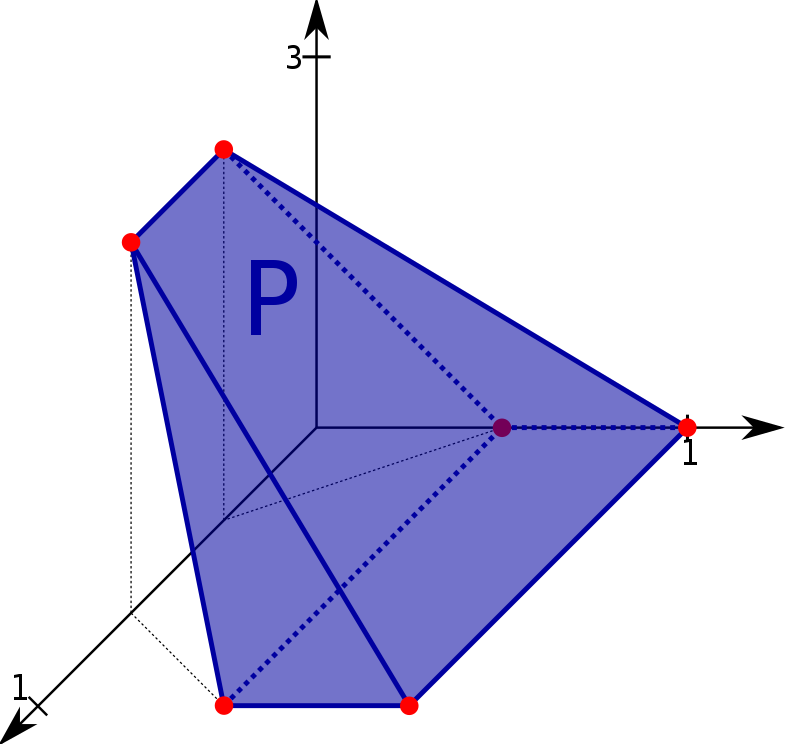
\includegraphics[width=0.7\textwidth]{region_factible_LP.png}
    \caption*{Una ilustración de una posible región factible en $\R^3$}
\end{figure}

Los bordes de la región factible están dados por los hiperplanos de la ecuación $Ax = b$. También es posible que la región no esté acotada: en cuyo caso puede pasar que el problema no tenga solución, y se pueda tomar valores de la función objetivo tan chicos como se desee.

\subsection{Método Simplex}

El \textit{método simplex} es un algoritmo para resolver problemas de programación lineal. Se basa en recorrer los vértices de la región factible (también llamada \textit{simplex}), ya que la solución óptima se debe encontrar en uno de ellos. En cada movimiento que realiza, la función objetivo no crece (e, idealmente, decrece). Como la cantidad de vértices crece exponencialmente con respecto a la cantidad de restricciones, el algoritmo es exponencial, y efectivamente corre lentamente para ciertos casos patológicos. No obstante, este algortimo es muy eficiente, y ampliamente utilizado, en la práctica.

\subsection{Reducciones}

Varios de los problemas de grafos que vimos en la materia se pueden reducir a programas lineales

\subsubsection{Flujo de costo mínimo}

Las restricciones de flujo de costo mínimo se dan en formato de programa lineal, así que la reducción es directa. Para una red de flujo $N = (V, E, u, b, c)$ Las ecuaciones e inecuaciones son:
\begin{gather*}
    \min{\sum_{vw \in E} c_{vw} x_{vw}} \\
    \begin{flalign*}
         &  & \sum_{w \in N^+(v)} x_{vw} - \sum_{w \in N^-(v)} x_{vw} & = b_v       &  & \forall v \in V  \\
         &  & x_{vw}                                                  & \geq l_{vw} &  & \forall vw \in E \\
         &  & x_{vw}                                                  & \leq u_{vw} &  & \forall vw \in E
    \end{flalign*}
\end{gather*}

\subsubsection{Flujo máximo}

Similarmente, se puede reducir el problema de flujo máximo a programación lineal\footnote{También se puede reducir ``pasando'' por flujo de costo mínimo, es decir, reducirlo primero a flujo de costo mínimo y luego a PL.}. Esto se logra de la siguiente manera:
\begin{gather*}
    \max{\sum_{v \in N^+(s)} x_{sv}} \\
    \begin{flalign*}
         &  & \sum_{w \in N^+(v)} x_{vw} - \sum_{w \in N^-(v)} x_{vw} & = 0         &  & \forall v \in V - \{s, t\} \\
         &  & x_{vw}                                                  & \geq 0      &  & \forall vw \in E           \\
         &  & x_{vw}                                                  & \leq u_{vw} &  & \forall vw \in E
    \end{flalign*}
\end{gather*}

\subsubsection{Camino mínimo}

Para un grafo pesado $V = (V, E, w)$ y un par de vértices $s, t \in V$, encontrar el camino mínimo entre $s$ y $t$ también se puede expresar como programa lineal, donde la variable $x_{uv}$ indica si una arista se utiliza ($x_{uv} = 1$) o no ($x_{uv} = 0$):
\begin{gather*}
    \max{\sum_{uv \in E} x_{uv} w_{uv}} \\
    \begin{flalign*}
         &  & \sum_{w \in N^-(t)} x_{vw}                              & = 1 &  &
         &  & \sum_{w \in N^+(v)} x_{vw} - \sum_{w \in N^-(v)} x_{vw} & = 0 &  & \forall v \in V - \{s, t\} \\
    \end{flalign*}
\end{gather*}

Esta reducción es equivalente a la reducción anterior de camino mínimo a flujo de costo mínimo. Las propiedades de la matriz de coeficientes garantizan que hay una solución óptima con $x_{ij} \in \{0, 1\}$.

\subsubsection{Árbol Generador Mínimo}

El problema de encontrar un AGM para un grafo pesado $G = (V, E, w)$ se puede expresar como el siguiente progama lineal:
\begin{gather*}
    \max{\sum_{uv \in E} x_{uv} w_{uv}} \\
    \begin{flalign*}
         &  & \sum_{uv \in E(S)} x_{vw} & \leq |S| - 1 &  & \forall S \subseteq V      \\
         &  & \sum_{uv \in E} x_{vw}    & = n - 1      &  & \forall v \in V - \{s, t\} \\
         &  & x_{vw}                    & \geq 0       &  & \forall vw \in E
    \end{flalign*}
\end{gather*}

También se puede demostrar que esta formulación tiene un óptimo entero. A pesar de que esta formulación tiene una cantidad exponencial de restricciones con respecto al tamaño del grafo original, se puede resolver en tiempo polinomial.

\subsection{P-Completitud}

No solo son los problemas anteriores los que se pueden reducir a PL: se puede demostrar que la programación lineal es P-Completo, esto es, cualquier problema resoluble en tiempo polinomial se puede reducir a él. En este sentido, es el problema ``más general'' entre ellos.

La teoría de clases de complejidad se estudia más en el \hyperref[capitulo-np-completitud]{siguiente capítulo}.

\subsection{Dualidad}

Para un problema de optimización que implica minimizar un valor, el \textit{problema dual} es uno que busca maximizarlo, y cuya solución es al menos tan grande como cualquier solución factible del primer problema (y viceversa para los problemas de maximización). Esto implica que si se encuentra una solución en la que coinciden, esta es mínima para el problema original.

Para la programación lineal, el problema dual de cualquier instancia es otro programa lineal. Si la instancia es:
$$\max{\{c^T x \mid x \in \R^n, Ax \leq b\}}$$

El programa lineal dual es:
$$\min{\{y^T b \mid y \in \R^m, y^T A \geq c\}}$$

\begin{theorem*}
    (Teorema de Dualidad Fuerte) Si un problema tiene una solución óptima, entonces el problema dual también la tiene, y sus valores coinciden.
\end{theorem*}
